\documentclass[12pt]{article}

\usepackage{sbc-template}

\usepackage{graphicx,url}

\usepackage[brazil]{babel}   
\usepackage{verbatim}
\usepackage{todonotes}
\usepackage{longtable}
\usepackage{amssymb}
\usepackage{amsmath}
\usepackage{float}
\usepackage{amsfonts}
\usepackage{algorithm, algpseudocode}
\usepackage{color}
\usepackage{minted}
\usepackage{url} 
%\usepackage[latin1]{inputenc}  
\usepackage[utf8]{inputenc}  
% UTF-8 encoding is recommended by ShareLaTex

     
\sloppy

\title{Projeto e Análise de Algoritmos -- \\ Caminhos Mínimos Utilizando Algoritmos de Dijkstra, Bellman-Ford, Floyd-Warshall, com detecção de Ciclos de Custo Negativo}
\author{Conrado C. Bicalho, Danilo S. Souza, Rodolfo L. M. Guimarães, Thiago Schons}

\address{Departamento de Computação -- Universidade Federal de Ouro Preto \\
 35.400-000 -- Ouro Preto - MG -- Brasil
 \email{\{conradobh, danilo.gdc, rodolfolabiapari, thiagoschons2\}@gmail.com}
 }




\begin{document} 

\maketitle

\begin{abstract}
This report aims to present the main algorithms for finding the shortest path between all pairs of nodes in a graph and these from all and all for everyone. The algorithms will be presented Dijkstra, Bellman-Ford, Floyd-Warshall with detection negative cost cycles, as well as their complexity, characteristics, implementation, results of experiments and final considerations.
\end{abstract}
     
\begin{resumo} 
Este relatório tem como principal objetivo apresentar os principais algoritmos para encontrar o caminho de custo mínimo entre todos pares de nós de um grafo sendo estes de todos e de todos para todos. Serão apresentados os algoritmos de Dijkstra, Bellman-Ford, Floyd-Warshall com detecção de ciclos de custo negativo, assim como suas complexidades, características, implementação, os resultados obtidos dos experimentos realizados e considerações finais.
\end{resumo}



\section{Introdução à Teoria de Grafos}

Segundo Netto \cite{netto2003grafos}, a definição de um grafo pode ser dada por uma estrutura $G=(V,E)$ onde $V$ é um conjunto discreto e não vazio de vértices e $E$ é uma família de elementos não vazios chamado de arestas, definidos em função dos elementos em $V$. Cada aresta tem um ou dois nós associados a ela e faz o papel de interligar suas extremidades. A Figura \ref{fig:naoponderado} exibe um exemplo de grafo com seus vértices e arestas.

\begin{figure}[H]
  \centering
    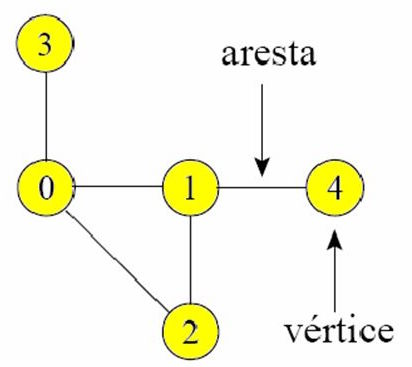
\includegraphics[width=0.3\textwidth]{img/naoponderado.jpg}
  \caption{Grafo simples exibindo arestas e vértices. Fonte: Autor.}
  \label{fig:naoponderado}
\end{figure}

Um grafo orientado $G=(V,E)$, também descrito como grafo direcionado ou dígrafo, consiste em um conjunto não vazio de vértices $V$ e um conjunto de arestas orientadas $E$. Cada aresta orientada está associada a um par ordenado de nós $(u, v)$ onde tal arco começa em $u$ e termina em $v$ como é exibido na Figura \ref{fig:orientado}.

\begin{figure}[H]
  \centering
    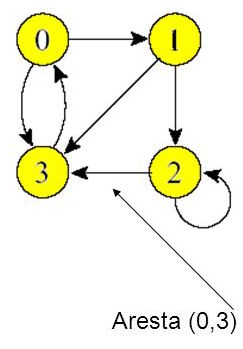
\includegraphics[width=0.25\textwidth]{img/ponderado.jpg}
  \caption{Exemplo simples de um grafo orientado. Fonte: Autor.}
  \label{fig:orientado}
\end{figure}

Tais arcos também podem ser ponderados sendo sua função peso $w(u, v) : E \rightarrow \mathbb{R}$ \cite{netto2003grafos}.


    
\subsection{Definição do Problema de Caminhos Mínimos de Única Origem} \label{sec:1todos}

	Segundo Cormen \cite{cormen2002algoritmos}, para definir o problema de caminho mínimo, deve considerar um grafo $G = (V, E)$ sem laços e valorado sobre os arcos por uma função peso $w : E \rightarrow \mathbb{R}$ mapeando arestas para pesos de valores reais sendo o peso $p = \left \langle v_{1}, v_{2}, \ldots, v_{k}  \right \rangle$ onde o somatório dos pesos de suas arestas constituintes 
    
    $$w(p) = \sum_{i=1}^{k} w(v_{i-1}, v_{i})$$
   
Portanto, o peso do caminho mais curto de $u$ até $v$ é definida por 
$$
	\delta(u, v) = 
	\begin{cases}
		\text{min}\{w(p):u\xrightarrow{p} v\} & \text{se existe um caminho de } u \text{ até } v\text{,}\\
		\infty & \text{em caso contrário.}
	\end{cases}
$$

Tais algoritmos se baseiam na propriedade de que um caminho mais curto entre dois vértices pode conter outros caminhos mais curtos em seu interior onde será explicado a seguir com mais detalhes.



\subsubsection{Prova da Subestrutura Ótima de um Caminho Mais Curto}

Cormen \cite{cormen2002algoritmos} continua explicando claramente como é o lema e a prova deste problema:

\textit{\textbf{Lema:}} Dado um grafo orientado ponderado $G = (V, E)$ com função peso $w : E \rightarrow \mathbb{R}$, seja $p = \left \langle v_{1}, v_{2}, \ldots, v_{k}\right \rangle$ um caminho mais curto do vértice $v_1$ até o vértice $v_k$ e, para quaisquer $i$ e $j$ tais que $1 \le i \le j \le k$, seja $p_{ij}= \left \langle v_{i}, v_{i + 1}, \ldots, v_{j}\right \rangle$ o subcaminho $p$ desde o vértice $v_i$ até o vértice $v_j$. Então, $p_{ij}$ é um caminho mais curto de $v_i$ e $v_j$.

\textit{\textbf{Prova:}} Quando realiza-se a decomposição do caminho $p$ em $v_1 \xrightarrow{p_{1i}} v_i \xrightarrow{p_{ij}} v_j \xrightarrow{p_{jk}} v_k$, então teremos $w(p) = w(p_{1i}) + w(p_{ij}) + w(p_{jk})$. Supondo que existisse um caminho $p^\prime_{ij}$ de $v_i$ até $v_j$ com peso $w(p^\prime_{ij}) < w(p_{ij})$. Então, $v_1 \xrightarrow{p_{1i}} v_i \xrightarrow{p^\prime_{ij}} v_j \xrightarrow{p_{jk}} v_k$ é um caminho de $v_1$ até $v_k$ cujo peso $w(p) = w(p_{1i}) + w(p^\prime_{ij}) + w(p_{jk})$ é menor que $w(p)$, o que contradiz a hipótese de que $p$ é um caminho mais curto de $v_1$ até $v_k$.



\subsubsection{Arestas de Peso Negativo}

Em algumas instâncias do problema, pode haver arestas cujo pesos são negativos. Deve-se ter em mente que se um grafo $G = (V,E)$ que não contenha nenhum ciclo de peso negativo acessível a partir da origem $s$, então para todo $v \in V$, o peso do caminho mais curto $\delta(s,v)$ permanece bem definido, mesmo tendo um valor negativo. Entretanto, caso exista um ciclo de peso negativo acessível, os pesos de caminhos mais curtos não serão bem definidos, permitindo uma série de caminhos mínimos entre $s$ e $v$, pelo fato de sempre ser possível encontrar um caminho que tenha menor custo fazendo ciclos repetidos. Existindo o ciclo negativo no caminho de $s$ até $v$, então $\delta(s,v) = - \infty$ \cite{cormen2002algoritmos}.

Um exemplo é exibido na Figura \ref{fig:negativo}. Tendo a premissa que o vértice de partida é o $s$, neste grafo, existe vértices que possuem caminho mínimo bem definido como os vértices $b$, $d$, $h$, $i$ e $j$ \footnote{Os vértices $h$, $i$ e $j$ são bem definidos pois todos são inacessíveis, tornando seu valor $+\infty$, ou seja, um valor bem definido segundo a definição do problema.} e vértices que não possuem caminho mínimo bem definido como os vértices $e$, $f$, $g$ no qual possuem pesos de caminhos mais curtos igual a $-\infty$.

\begin{figure}[H]
  \centering
    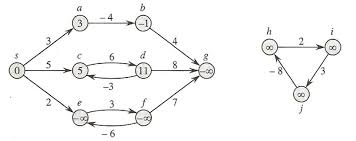
\includegraphics[width=0.8\textwidth]{img/negativo2.jpeg}
  \caption{Exemplo simples de um grafo com arestas de peso negativo. Fonte: \cite{cormen2002algoritmos}.}
  \label{fig:negativo}
\end{figure}

O Algoritmo de Dijkstra por exemplo, necessita que todos os arcos devem ser não negativos para sua execução de forma correta. Já algoritmos como o Bellman-Ford e Floyd-Warshall permitem arestas de peso negativo no grafo de entrada e produzem resposta correta enquanto nenhum ciclo de peso negativo é acessível a partir da origem. 

Os exemplos dados até agora está relacionado a apenas ao problema de menor caminho de uma única origem para todos os vértices. Mas além desta, existe uma variação  que deste problema que em como propósito encontra o caminho mais curto de todos os vértices para todos os vértices utilizando um único algoritmo sem utilizar repetições sucessivas dele. Ela é descrita a seguir.



\subsection{Caminhos mais Curtos de Todos para Todos}

Diferentemente do método citado anteriormente, que procura o caminho mínimo de todos os vértices a partir de uma única fonte, os algoritmos todos para todos, calculam a distância mínima de todos os pares de vértices de um grafo.

Tal como dito na Seção \ref{sec:1todos}, tem-se um grafo orientado ponderado com sua função peso que mapeia as arestas como pesos de valores reais. Entretanto, deseja-se encontrar o caminho mais curto entre todos os pares de vértices $u,v \in V$ onde o peso de um caminho é a soma dos pesos de suas arestas constituintes. Este problema também pode ser resolvido utilizando um algoritmo de caminho mínimo um para todos $|V|$ vezes, uma para cada vértice de origem, mas existem algoritmos específicos para a resolução deste.

Naturalmente, sua estrutura de dados é lidada como uma matriz de adjacência onde é exibido os valores de todos para todos de acordo com sua linha e colina. Supondo que existem $|V|$ vértices e enumerados de forma crescente e contínua, uma matriz de entrada seria $W\ n \times n$ representando os peso das arestas do grafo orientado de $n$ vértices. Isto é, $W = (w_{ij})$ onde 
$$
w_{ij} = 
	\begin{cases}
    	0 & \mbox{se } i = j, \\
        \mbox{o peso da aresta orientada } (i, j) & \mbox{se } i \neq j \mbox{ e } (i, j) \in E, \\
        \infty & \mbox{se } i \neq j \mbox{ e } (i, j) \notin E.
    \end{cases}
$$

Arestas negativas também são permitidas mas com a continuidade da restrição de ciclos negativos. 



\subsection{Variantes do Problema}

Tal como descrito ao longo do texto, foram exibidas duas variantes do problema de caminho mínimo: a de caminho mais curto de uma única origem; e de todos para todos. Mas além destes, é possível obter outras variantes deste problema sem perder sua natureza. Seriam as outras variantes: o caminho mais curto de destino único; e de par único.

	O problema de destino único busca encontrar todas as distâncias de todos os vértices para um determinado destino e de par único são problemas que desejam encontrar a menor distância entre dois pontos específicos do grafo.



\subsection{Aplicações}

	Estes problemas de uma única origem envolvem naturalmente problemas relacionados com sequências de decisões (escolhas de itinerários ao longo de uma viagem ou traçado de uma estratégia em um problema de investimentos). Sendo assim, trata-se de decisões envolvendo alguma forma de custo a ser minimizado.
    
    Já o problema de todos para todos seria útil numa possível elaboração de uma tabela de distância entre todos os pares de cidades de um certa região para um atlas rodoviário.



\section{Os Algoritmos}

Nesta seção, será descrito como a literatura aborda os algoritmos, suas principais características e como foram implementados junto com a análise de sua complexidade assintótica.


\subsection{Considerações de Projeto e Análise}

Para que o usuário fique ciente de algumas decisões utilizadas na implementação, esta seção tratará de alguns detalhes que são importantes para compreender o projeto dos algoritmos:

\begin{itemize}
	\item Alguns algoritmos implementados tratam o `infinito' como: o maior peso encontradas das arestas multiplicado por ele mesmo. \newline
    	Isso pois, ele será o maior valor e, comparado a todos os outros valores, ele é considerado infinito.
        
    \item Nenhum algoritmo faz teste de verificação de entradas inválidas. \newline
    	Isso foi necessário pela tempo de implementação e testes a serem realizados. É necessário que todas as instâncias sejam compatíveis para cada um dos algoritmo, ou seja, não deve-se colocar uma instância com peso negativo no Algoritmo do Dijkstra pois ele não avisará erro e tentará executar normalmente. 
        
    \item Foi executado em todos os algoritmos analisadores de código estáticos e dinâmicos. Executou-se primeiramente o Clang Static Analyzer e em seguida o Valgrind. Com exceção do Algoritmo de Bellman Ford, todos retornaram sucesso nas análises.\newline 
    O Algoritmo de Belmman Ford encontrou-se o seguinte \textit{warning} que não fora resolvido:
\begin{verbatim}
scan-build: Using '/Users/pripyat/clang/bin/clang' for static analysis
main.c:147:18: warning: Potential memory leak
                          * maior_peso = -1;
                          ~~~~~~~~~~~~~^~~~
1 warning generated.
scan-build: 1 bug found.
\end{verbatim}
    Mas em conversa com o Professor orietador da disciplina, este não é um problema a se preocupar podendo continuar com a execução dos testes.
        
       
\end{itemize}


\subsection{Ambiente de \textit{Hardware} e \textit{Software }Utilizado}

A descrição do ambiente de testes é descrito abaixo.

\begin{table}[H]
	\caption{Tabela com as informações de ambiente de execução do trabalho realizado.}
	\centering
    \begin{tabular}{l|l}
    \hline
    \textbf{Item}                & \textbf{Descrição} \\ \hline \hline
    Processador         & 1 Processador Intel Core i7 - 2,9 GHz         \\
    Núcleos             & 4 Núcleos \\
    Cache L2 (por Núcleo) & 256 KB \\
    Cache L3            & 4 MB \\
    Memória RAM         & 10 GB DDR3        \\
    Arquitetura         & Arquitetura de von Neumann         \\
    Sistema Operacional & OS X 10.11.4 (15E65)         \\
    Versão do Kernel    & Darwin 15.4.0 \\
    Compilador          & Apple LLVM version 7.3.0 (clang-703.0.31)         \\\hline
    \end{tabular}
\end{table}

\subsection{Relaxamento}

Cormen \cite{cormen2002algoritmos} também explica a técnica de relaxamento. Os algoritmos possuem a técnica de relaxamento onde para cada vértice $v \in V$, mantém-se um atributo $d[v]$, chamado de estimativa de caminho mais curto, que é o limite superior sobre o peso do caminho mais curto entre $s$ e $v$. Assim, como primeiro passo, a estima de distância de cada vértice é infinito, já que o algoritmo não sabe de antemão qual é o caminho mais curto até cada um deles\footnote{Com exceção do no de partida $s$ que a distância para ele mesmo é zero.}. 
Faz-se uma estimativa pessimista inicial para o caminho mínimo até cada vértice: $d(v)=\infty$.

O processo de relaxar uma aresta $(u,v)$ consiste em testar alguma forma de melhorar o caminho mais curto para $v$ encontrado até agora por outros caminhos intermediários que utilizem $u$. Um relaxamento realiza a alteração dos valores conhecidos das distâncias atuais atualizando-os para novos valores de acordo com os caminhos intermediários testados atualizando o novo predecessor de $v$ como é exibido na Figura \ref{fig:relaxamento}.

\begin{figure}[H]
  \centering
    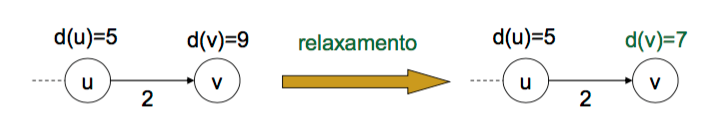
\includegraphics[width=1\textwidth]{img/relaxamento.png}
  \caption{Exemplo de um relaxamento de uma aresta. Fonte: \protect\url{http://wiki.icmc.usp.br/images/b/b4/7._1GrafosCaminhosLA(Graca).pdf}}
  \label{fig:relaxamento}
\end{figure}
%http://wiki.icmc.usp.br/images/b/b4/7._1GrafosCaminhosLA(Graca).pdf

Nesta imagem, existe um caminho já conhecido que utiliza a aresta $(u,v)$ com custo de 9 unidades. O relaxamento consiste em encontrar outro caminho que utiliza um custo menor que o atual que no caso foi encontrado uma aresta com peso $2$ partindo de $d[u]=5$ totalizando $d[v]=7$, ou seja, um caminho intermediário menor que o atual. O novo valor é atualizado e o processamento do algoritmo continua até que todos sejam analisados.

\subsection{Algoritmo Bellman-Ford}

De acordo com Cormen \cite{cormen2002algoritmos}, tal algoritmo se baseia em algoritmos independentes
criados por Bellman e Ford. Ele resolve o problema de caminhos mais curtos de uma única origem no caso mais geral\footnote{Caso que é permitido arestas com valores negativos.}. Ao final, o algoritmo verifica se existe ou não um ciclo de peso negativo acessível a partir da origem. Não existe solução se e somente se existe um ciclo negativo a partir da origem. Caso contrário, retorna os caminhos mais curtos e seus pesos.

Utiliza a técnica de relaxamento já citada reduzindo progressivamente o peso do caminho da origem até $v \in V$ até alcançar o peso real do caminho mais curto.


\begin{algorithm}[H]
\caption{Bellman-Ford}\label{alg:d}
\begin{algorithmic}[1]
\Procedure{Bellman-Ford}{$G, w, s$}
	\State INICIALIZA-UNICA-FONTE(G, s);
    \For{$i \gets 1, |V[G]| - 1$}
      \For{cada aresta $(u,v) \in E[G]$}
	      \State RELAXA(u, v, w);
      \EndFor
    \EndFor
    
    \For{cada aresta $(u,v) \in E[G]$}
      \If{$d[v] > d[u] + w(u,v)$}
	      \State \textbf{return} FALSE;
      \EndIf
    \EndFor
    \State \textbf{return} TRUE;
\EndProcedure
\end{algorithmic}
\end{algorithm}

Este pseudocódigo possui detector de ciclos negativos. Seu comando \texttt{for} situado na linha 9 realiza a verificação de valores de caminhos de menor custo que não serão bem definidos.


\subsubsection{Análise do Algoritmo}

Após a inicialização o algoritmo realiza $|V| - 1$ passagens sobre as arestas do grafo. Cada passagem consiste em relaxar cada aresta do grafo uma vez. Depois de fazer $|V| - 1$ passagens, é realizado a procura de um ciclo negativo.

Sendo assim, é executado no tempo $\mathcal{O}(VE)$ podendo então ser comparado a $\mathcal{O}(n^2)$ no pior caso. Isso pois a inicialização demora $\Theta(V)$, em seguida cada uma das $|V| - 1$ passagens sobre as arestas demoram $\Theta(E)$, e o loop final que demora $\mathcal{O}(E)$.



\subsection{Algoritmo de Dijkstra} \label{sec:firstpage}

O algoritmo de Dijkstra surgiu em 1959 e resolve o problema de caminhos mais curtos de uma única origem em um grafo orientado de arestas com pesos não negativos. Em razão disso, deve-se supor sempre que $w(u, v) \geq 0$ para cada aresta $(u,v) \in E$.

O algoritmo mantém um conjunto $S$ de vértices cujo pesos finais de caminhos mais curtos desde a origem já foram determinados. Seu diferencial é que ele seleciona repetidamente o vértice $u \geq V - S$ com a estimativa mínima de caminhos mais curtos, adiciona $u$ a $S$ e relaxa todas as arestas que saem de $u$ \cite{cormen2002algoritmos}.

Ele escolhe sempre o vértice `mais leve' ou `mais próximo' em $V - S$ para adicionar ao conjunto $S$ e com isso utiliza-se a estratégia gulosa em sua execução.

\begin{algorithm}[H]
\caption{Dijkstra}\label{alg:d}
\begin{algorithmic}[1]
\Procedure{Dijkstra}{$G, w, s$}
	\State INICIALIZA-UNICA-FONTE(G, s);
   \State $S\gets \emptyset$;
   \State $Q\gets V[G]$;
   \While{$Q\not=\emptyset$}
      \State $u\gets$ RETIRA-MINIMO(Q);
      \State $S\gets S \cup \{u\}$;
      \For{cada vértice $v \in Adj[u]$}
	      \State RELAXA(u, v, w);
      \EndFor
   \EndWhile\label{euclidendwhile}
\EndProcedure
\end{algorithmic}
\end{algorithm}


Este algoritmo não possui detector de ciclo negativos. Aliás, como já mencionado, este algoritmo não suporta arestas negativas.


\subsubsection{Análise do Algoritmo}

Primeiramente ele realiza uma inicialização (linha 2) das arestas sendo sua complexidade  $\mathcal{O}(E)$.

Em seguida, ele realiza uma remoção de cada nó que ele opera (linha 4 - 6) e logo depois realiza o relaxamento para cada item na franja (linha 8 e 9). Isso pode ser considerado $\mathcal{O}(V\log V)$.

Assim, o algoritmo, no pior caso tem complexidade de tempo $\mathcal{O}(E + V\log V)$.

\subsection{Algoritmo Floyd-Warshall}

Desenvolvido por Bernard Roy, Stephen Warshall e Robert Floyd, o algoritmo utiliza uma formulação de programação dinâmica para resolver o problema de caminhos mais curtos de todos os pares de grafos \cite{cormen2002algoritmos}.


\begin{algorithm}[H]
\caption{Floyd-Warshall}\label{alg:fw}
\begin{algorithmic}[1]
\Procedure{Floyd-Warshall}{$W$}
	\State $n \gets linhas[W]$;
   \State $D\gets W$;
   \For{$k \gets 1, n$}
     \For{$i \gets 1, n$}
       \For{$j \gets 1, n$}
           \State $d^k_{ij} \gets min(d^{k-1}_{ij}, d^{k-1}_{ik} + d^{k-1}_{kj})$;
       \EndFor
     \EndFor
   \EndFor
   \State \textbf{return} $D$;
\EndProcedure
\end{algorithmic}
\end{algorithm}



Além da matriz de pesos, também é necessário uma matriz de mesma dimensão que armazenará os predecessores de cada vértice que no pseudocódigo foi nomeada de $D$. Inicialmente, ela é preenchida com os valores das arestas obtidas dos dados de entrada e serão modificadas a cada relaxamento realizado ao longo da execução do algoritmo \cite{cormen2002algoritmos}.

Este algoritmo assume que sua entrada não inclui nenhum ciclo negativo.

\subsection{Análise do Algoritmo}

Cada laço \texttt{for} deste algoritmo pode ser entendido como um somatório de um mesmo valor constante supondo que a operação da linha 7 é uma operação elementar. Assim, temos que sua complexidade é dada por

    $$\sum_{k=1}^{n}\sum_{i=1}^{n}\sum_{j=1}^{n}1$$
    
Já que cada somatório é a repetição de o valor 1 $n$ vezes, então este pode ser convertido para

$$n\sum_{k=1}^{n}\sum_{i=1}^{n}1$$

Portanto

$$n^3$$

Então, sua complexidade assintótica `pode ser descrita como $\mathcal{O}(n^3)$.



\section{Experimentos}

Para a realização dos experimentos, utilizou-se de um \textit{script} em \textit{Shell} para a execução dos testes de forma controlada e autônoma. Para cada iteração, foi analisado o tempo de execução e assim comparado com os demais algoritmos.

Para tal teste, utilizou-se de 3 (três) instâncias, entretanto, para que a execução de grafos com peso negativo sejam testados também, foi selecionado uma das instâncias e suas arestas foram alteradas para que se comporte como um grafo com arestas negativas, totalizando 4 instâncias. São elas: \textit{rome99.gr}, \textit{rg300\_4730.gr}, \textit{rg300\_768\_floyd.gr}, \textit{rg300\_768\_floyd-n.gr} sendo a última modificada.

Isso foi necessário pois as instâncias com arestas de peso negativo encontradas na literatura eram grandes e colocaria o projeto em risco já que executar 20 (vinte) iterações de um problema poderia levar tempo demais para logo analisar, gerar gráficos e tabelas e a conclusão deste.

Para cada instância foi executada 20 (vinte) vezes no mesmo ambiente de testes para que os dados tenham uma média de tempo confiante.

Todos os resultados de cada iteração são exibido em anexo neste relatório, junto com cada algoritmo implementado.



\subsection{Formato de Saída}

Como meio de tornar o algoritmo útil, decidiu-se que ele teria como saída de arquivo a impressão de todos os caminhos por ele analisados (que no caso é todos para todos). O formato deste está da seguinte forma:

\begin{verbatim}
[origem,destino](distancia) caminho_origem_ate_destino
\end{verbatim}

Um exemplo e exibido a seguir:

\begin{verbatim}
[1,2](8) 1 4 2
[1,3](9) 1 4 2 3
[1,4](5) 1 4
\end{verbatim}


\subsection{Análise de Tempo do Problema de Caminho Mínimo de Todos para Todos}

Para melhor visualização dos resultados, foram desenvolvidos tabelas e gráficos.

Abaixo é exibido a tabela com os valores médios de cada algoritmo sobre cada instância. As tabelas com os valores de cada iteração é exibido em anexo no relatório.

Deve-se notar que a instância \textit{rg300\_768\_floyd-n.gr} é a instância que foi alterada pelo grupo para que se comporte como um grafo com arestas de peso negativo e por isso, foi adicionado um \textit{-n} no seu nome para diferenciar das outras. 

Como já dito anteriormente, o Algoritmo de Dijkstra não suporta grafos com arestas negativas e por isso, seus dados sobre esta instância não se aplicam.

\begin{table}[H]
	\centering
	\caption{Tabela com os valores de tempo médio de cada algoritmo nas quatro instâncias com o objetivo de obter caminhos mínimos de todos para todos.}
    \begin{tabular}{l|lll}
    \hline
    \textbf{Instância} & \textbf{Bellman-Ford (s)} & \textbf{Dijkstra (s)} & \textbf{Ford-Warshall (s)} \\ \hline \hline
   \textit{ rome99.gr}         & 420.0757                           & 93.59347                          & 149.3292                            \\
   \textit{ rg300\_4730.gr}         & 1.788467                           & 0.11464                          & 0.118966                            \\
   \textit{ rg300\_768\_floyd.gr}         & 0.294253                           & 0.094997                          & 0.116002                            \\
   \textit{ rg300\_768\_floyd-n.gr}    & 0.289948  & Não se aplica.                              & 0.098479                            \\ \hline
    \end{tabular}
\end{table}


A Figura \ref{fig:rome} exibe um gráfico comparando os resultados de cada algoritmo sobre a instância \textit{rome99.gr}.

\begin{figure}[H]
  \centering
    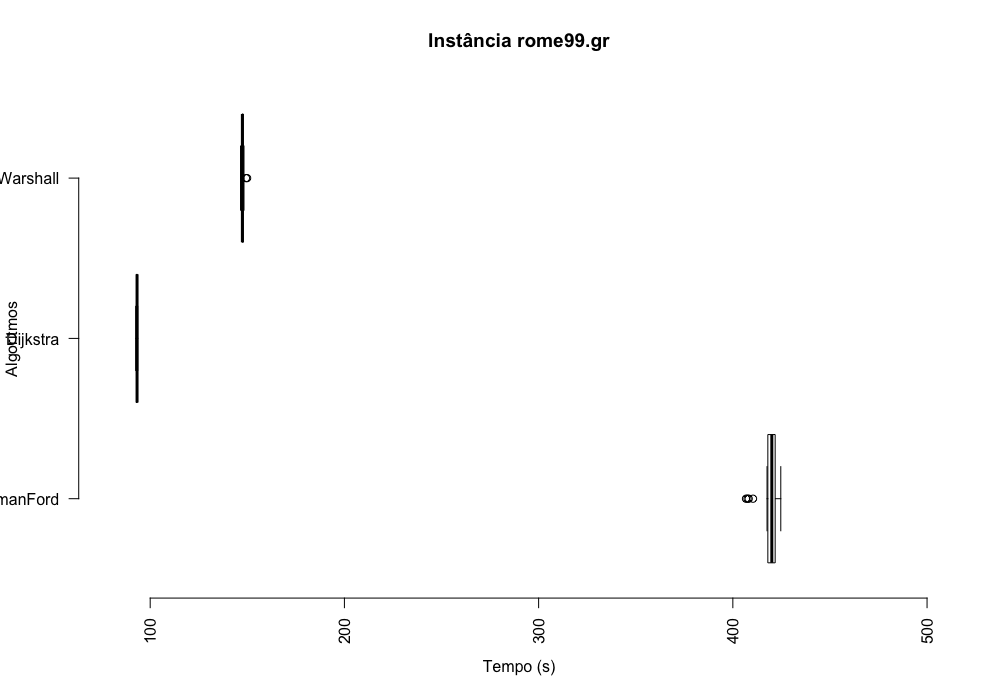
\includegraphics[width=1\textwidth]{img/rome99.png}
  \caption{Tempo de execução de cada algoritmo sobre a instância \textit{rome99.gr}. Fonte: Autor.}
  \label{fig:rome}
\end{figure}


A Figura \ref{fig:rg300_4730} exibe um gráfico comparando os resultados de cada algoritmo sobre a instância \textit{ rg300\_4730.gr}.

\begin{figure}[H]
  \centering
    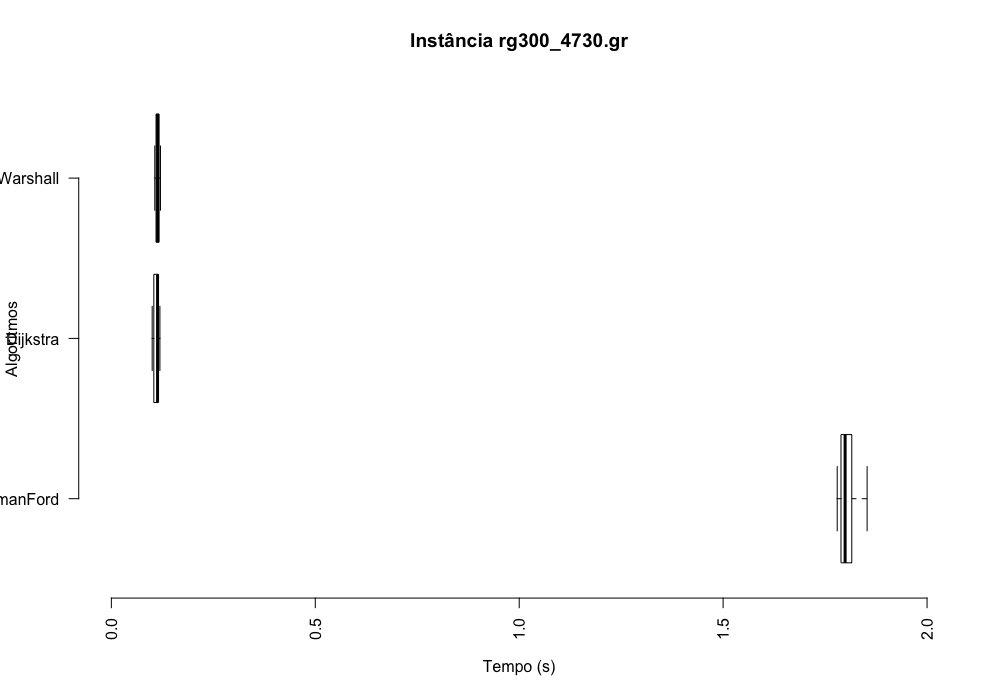
\includegraphics[width=1\textwidth]{img/rg300_4730.png}
  \caption{Tempo de execução de cada algoritmo sobre a instância \textit{rg300\_4730.gr}. Fonte: Autor.}
  \label{fig:rg300_4730}
\end{figure}



A Figura \ref{fig:rg300_768_floyd} exibe um gráfico comparando os resultados de cada algoritmo sobre a instância \textit{ rg300\_768\_floyd.gr}.

\begin{figure}[H]
  \centering
    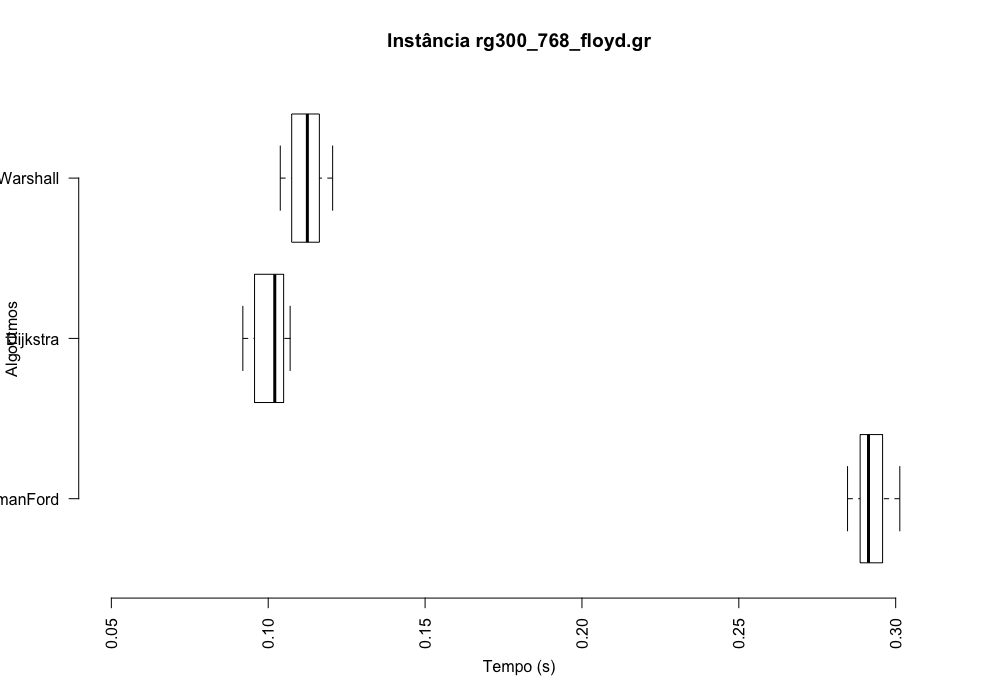
\includegraphics[width=1\textwidth]{img/rg300_768_floyd.png}
  \caption{Tempo de execução de cada algoritmo sobre a instância \textit{rg300\_768\_floyd.gr}. Fonte: Autor.}
  \label{fig:rg300_768_floyd}
\end{figure}


A Figura \ref{fig:rg300_768_floyd_n} exibe um gráfico comparando os resultados de cada algoritmo sobre a instância \textit{ rg300\_768\_floyd-n.gr}. Lembrando que o Algoritmo de Dijkstra não opera sobre grafos que tenham arestas com peso negativo.

\begin{figure}[H]
  \centering
    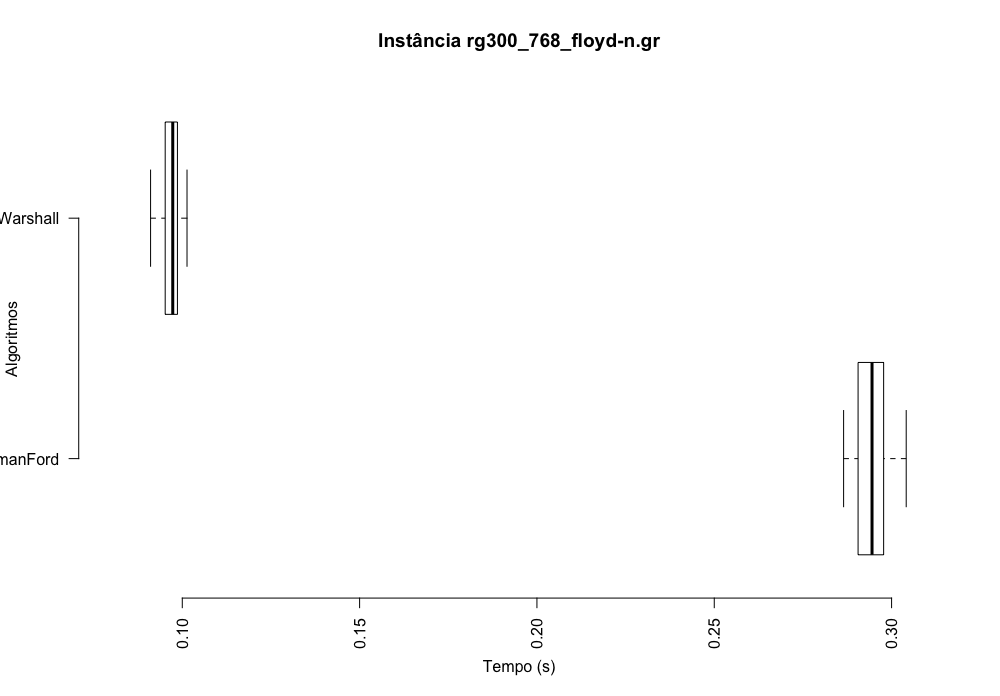
\includegraphics[width=1\textwidth]{img/rg300_768_floyd-n_gr.png}
  \caption{Tempo de execução de cada algoritmo sobre a instância com arestas negativas \textit{rg300\_768\_floyd-n.gr}. Fonte: Autor.}
  \label{fig:rg300_768_floyd_n}
\end{figure}


\subsection{Conclusão}\label{sec:figs}


Primeiramente, algo interessante a se notar é que o problema de caminhos mínimos também está relacionado a programação linear. É possível reduzir um caso especial de programação linear ao fato de encontrar caminhos mais curtos a partir de uma única origem. Tal problema pode ser resolvido com algoritmo de Bellman-Ford, sendo assim resolvendo também o problema de programação linear \cite{cormen2002algoritmos}.

Os resultados foram expressos por meio de tabelas e gráficos (Boxplot) pelo fato de ambos serem itens fundamentais para a compreensão do leitor do relatório. Realizou-se 20 iterações de teste devido ao tempo computacional elevado pelo tamanho das instâncias utilizadas assim como a complexidade dos algoritmos. 

Em termos de implementação, todos os códigos possuem grande facilidade de implementação. Principalmente o Algoritmo Floyd Warshall que se baseia numa simples estratégia que utiliza três \texttt{for} aninhado e realiza uma única verificação e atribuição dentro deles. Entretanto, em análise assintótica sua facilidade se torna um problema.

Na análise assintótica houve uma grande disputa entre o Bellman Ford e Dijkstra. O Algoritmo de Floyd Warshall ficou fora dessa disputa por ser de complexidade de tempo  $\mathcal{O}(n^3)$ e o Bellman tem complexidade  $\mathcal{O}(n^2)$ e o Dijkstra $\mathcal{O}(E + V \log V)$ no pior caso. O algoritmo Dijkstra teve sucesso sua complexidade de tempo ser menor que todos os outros. A estrutura utilizada nele foi projetada pelos integrantes dos grupos. Também houve vários problemas com \textit{Warnings} que o compilador do Bellman Ford relatou que, como já mencionado, o grupo não soube explicar a origem.

\section{Algoritmos}
\subsection{Shell Script para Execução Autônoma}

\begin{minted}
[
frame=lines,
framesep=2mm,
tabsize=3,
breaklines=true,
baselinestretch=1.2,
fontsize=\scriptsize,
linenos
]{shell}
#!/bin/bash

# Questiona quantas iteracoes
echo "Quantas iteracoes?"
read quantidade_iteracoes;
echo

# Remove dados de iteracoes passadas
eval "rm saida*"
eval "rm tempo*"

# Compila os arquivos novamente
eval "gcc bellman/bellman.c -o bellman/bellman"
eval "gcc floyd/floyd.c -o floyd/floyd"
eval "gcc dijkstra/dijkstra.c -o dijkstra/dijkstra"

# Vetor de instancias
instancias=( rome99.gr rg300_4730.gr rg300_768_floyd.gr rg300_768_floyd-n.gr )

# Algoritmos a serem testados
algoritmos=( bellman dijkstra floyd )

# Execucoes
for algoritmo in "${algoritmos[@]}"
do
	echo $algoritmo

  for instancia in "${instancias[@]}"
  do
  	echo $instancia

    for (( i = 0; i < "$quantidade_iteracoes"; i++ )); do
      echo "$i"

      cmd="./$algoritmo/$algoritmo $instancia"
      date
      echo $cmd
      $cmd
    done
    echo

  done
  echo

done
\end{minted}



\subsection{Bellman Ford em C}
\begin{minted}
[
frame=lines,
framesep=2mm,
tabsize=3,
breaklines=true,
baselinestretch=1.2,
fontsize=\scriptsize,
linenos
]{C}
/*
 * Trabalho de Projeto e Análise de Algoritmo
 * Mestrado em Ciência da Computação - Turma 16.1
 *
 * Alunos (nome, matricula, e-mail):
 * 	Conrado
 * 	Danilo Santos Souza                16.1.10149 - danilo.gdc@gmail.com
 * 	Rodolfo Labiapari Mansur Guimarães 16.1.10163 - rodolfolabiapari@gmail.com
 * 	Thiago Schons                      16.1.10186 - thiagoschons2@gmail.com
 *
 * Este arquivo executa o Algoritmo de Bellman Ford.
 *
 *
 * Para executar o arquivo utilize o comando:
 * 	"./nomeDoPrograma benchmark"
 *
 *
 * Saída está descrita da seguinte forma: [origem, destino](distancia) caminho
 * Abaixo é exibido um exemplo
 * [1,2](8) 1 4 2
 * [1,3](9) 1 4 2 3
 * [1,4](5) 1 4
 */
#include <stdio.h>
#include <stdlib.h>
#include <math.h>
#include <time.h>

/*
 * Estrutura que armazena os valores de uma aresta
 */
typedef struct Edges {
	int origem;
	int destino;
	float peso;
} Edge;


/*
 * Utilizou-se de uma pilha para imprimir a ordem de saída na forma
 * origem -> destino. O algoritmo naturalmente imprime de forma inversa, e por
 * isso necessitou de uma pilha.
 */
typedef struct Pilhas {
    int noh;
    struct Pilhas * prox;
} Pilha;


/*
 * Procedimento de empilhar um novo item na pilha
 */
void pushPilha (Pilha ** s, int noh) {
	Pilha * noh_pilha = calloc(1, sizeof(Pilha));

	noh_pilha->noh = noh;
	noh_pilha->prox = *s;

	*s = noh_pilha;
}

/*
 * Procedimento de retirar um item da pilha
 */
int popPilha (Pilha ** s) {
	int retorno;
	Pilha * proximo;

	if (s != NULL) {
		retorno = (*s)->noh;
		proximo = (*s)->prox;

		free(*s);

		*s = proximo;

		return retorno;

	} else {
		return -1;
	}
}

/*
 * Procedimento que realiza a retirada dos dados da pilha imprimindo cada um
 * deles.
 */
void imprimePilha(Pilha * s, FILE * f) {

	if (s == NULL) {
		return;
	} else {

		while (s != NULL) {
			fprintf(f, " %d", s->noh);
			popPilha(&s);
		}
	}
	fprintf(f, "\n");
}


/*
 * Procedimento que retira todos os itens da pilha
 */
void esvaziaPilha(Pilha * s) {

	Pilha * atual, * proximo;

	if (s == NULL) {
		return;
	} else {
		atual = s;
		proximo = s->prox;

		while (proximo != NULL) {
			free (atual);

			atual = proximo;
			proximo = atual->prox;
		}

		free (atual);
	}
}

/*
 * Procedimento responsável por ler o arquivo e recolher as informações do
 * grafo nele contido.
 */
void le_arquivo(char * diretorio, Edge ** lista_arestas, int * vertices, int * arestas, int * maior_peso) {

	// Define o ponteiro pro arquivo em modo de leitura
	FILE * bench = fopen(diretorio, "r");

	int i = 0, origem_tmp = 0, destino_tmp = 0, peso_tmp = 0;
	char criou_lista = 0;

	// Contador de quantas arestas foram lidas
	int count_arestas = 0;


	// Lê do arquivo o comando da linha
	char comando = fgetc(bench);

	// Enquando não for final de arquivo
	while (comando != EOF) {

		// Verifica qual comando é o comando
		switch (comando) {
			// Comentários serão ignorados
			case 'c':
					while(fgetc(bench) != '\n') ;

				break;

			// Informações iniciais do grafo como número de vértices e
				// arestas
			case 'p':
				if (!(fgetc(bench) == ' ')) {
					printf("Erro na inicializacao!\n");
					exit(2);
				}
				if (!(fgetc(bench) == 's')) {
					printf("Erro na inicializacao!\n");
					exit(2);
				}
				if (!(fgetc(bench) == 'p')) {
					printf("Erro na inicializacao!\n");
					exit(2);
				}

				// Le o número de vertices e arestas
				fscanf(bench, "%d %d", vertices, arestas);

				// Flag indicando que a lista foi criada
				criou_lista = 1;

				// Variável indicando o maior peso encontrado no momento
				* maior_peso = -1;

				// Aloca a quantidade exata de arestas lida previamente pelo
					// arquivo
				*lista_arestas = calloc(*arestas, sizeof(Edge));

				break;

			case 'a':

				// Verifica a flag de criaçao da lista
				if (criou_lista == 0) {
					printf("Lista não criada!\n");
					exit(-1);
				}

				// Lê a aresta
				fscanf(bench, "%d %d %d", &origem_tmp, &destino_tmp, &peso_tmp);

				// Atribou as informações no vetor, na primeira posição vazia
				(*lista_arestas)[count_arestas].origem  = origem_tmp;
				(*lista_arestas)[count_arestas].destino = destino_tmp;
				(*lista_arestas)[count_arestas].peso    = peso_tmp;

				// Verifica se encontrou algum peso maior que o já encontrado
				if (peso_tmp > * maior_peso)
					* maior_peso = peso_tmp;

				// Le a aresta e seu valor
				count_arestas++;

				// Quebra a linha
				fgetc(bench);

				break;

			default:
				break;
		}

		// Le o proximo comando
		comando = fgetc(bench);
	} //while

	// Verifica se a contagem de leitura de arestas foi realmente exato
	if ((criou_lista == 0) || (count_arestas != *arestas)) {
		printf("Numero de arestas está incorreto em relação ao arquivo.\n");
		exit(-1);
	}

	// Para a representação do infinito, utilizou-se o maior peso encontrado ao
	// quadrado
	*maior_peso = *maior_peso * *maior_peso;

	// Fecha o arquivo aberto
	fclose(bench);
}

/*
 * Procedimento simples para impressão de das distâncias encontradas
 */
void imprimeDistancias(int * distancia, int vertices) {
	int i;
	printf("\n\n\n");
	for (i = 0; i < vertices; i++)  {
		printf("%4d ", i);
	}

	printf("\n");

	for (i = 0; i < vertices; i++)  {
		printf("%4d ", distancia[i]);
	}

}

/*
 * Procedimento que imprime os predecessores de cada vértice
 */
void imprimePredecessores(int * predecessor, int vertices) {
	int i;
	printf("\n\n");
	for (i = 0; i < vertices; i++)  {
		printf("%4d ", i);
	}

	printf("\n");

	for (i = 0; i < vertices; i++)  {
		printf("%4d ", predecessor[i]);
	}
}


/*
 * Algoritmo De Belmman-Ford.
 * Baseado no pseudocódigo do livro do Cormen.
 */
void bellmanFord(Edge * lista_arestas, int ** distancia, int ** predecessor, int vertices, int arestas, int origem, int maior_peso) {
	int i, j, peso;

	// Aloca um vetor de distâncias e de predecessores temporários
	int * distancia_temp   = calloc(vertices, sizeof(int));
	int * predecessor_temp = calloc(vertices, sizeof(int));

	// Inicializa os vetores temporários com
	for (i = 0; i < vertices; i++) {
		// Distância como 'infinito'
		distancia_temp[i] = maior_peso;
		// predecessor como inexistente no momento
		predecessor_temp[i] = -1;
	}

	// Informa que a distância da origem pra ela mesma é 0
	distancia_temp[origem - 1] = 0;

	// Executa o algoritmo
	for (i = 0; i < vertices; i++) {
		for (j = 0; j < arestas; j++) {
			peso = lista_arestas[j].peso;

			// Verifica se existe uma distância menor por outro caminho
			if (distancia_temp[lista_arestas[j].origem - 1] + peso < distancia_temp[lista_arestas[j].destino - 1] ){
				// Se sim, realiza as atualizações
				distancia_temp[lista_arestas[j].destino - 1] = distancia_temp[lista_arestas[j].origem - 1] + peso;

				predecessor_temp[lista_arestas[j].destino - 1] = lista_arestas[j].origem - 1;
			}
		}
	}

	// Realiza uma verificação final de ciclos negativos
	for (i = 0; i < arestas; i++) {
		peso = lista_arestas[i].peso;

		if (distancia_temp[lista_arestas[i].origem - 1] + peso < distancia_temp[lista_arestas[i].destino - 1]) {
			printf("[%d,%d] Graph contains a negative-weight cycle\n", lista_arestas[i].origem, lista_arestas[i].destino);
			exit(-1);
		}
	}

	// Retorna os vetores criados
	*distancia = distancia_temp;
	*predecessor = predecessor_temp;
}



/*
 * Procedimento final que imprime o caminho para melhor visualização do usuário
 * bem como o valor total da distância.
 */
void imprimeTodosCaminhos(FILE * file, int * distancia, int * predecessor, int vertices, int origem) {

	int anterior, i;

	Pilha * stack;

	for(i = 0; i < vertices; i++) {
		if (i != origem -1) {
			if (predecessor[i] != -1) {

				fprintf(file, "[%d,%d](%d)", origem, i + 1, distancia[i]);

				stack = NULL;

				pushPilha(&stack, i + 1);

				anterior = predecessor[i];
				while(anterior != origem - 1) {
					pushPilha(&stack, anterior + 1);

					anterior = predecessor[anterior];
				}

				fprintf(file, " %d", origem);

				imprimePilha(stack, file);
			}
		}
	}
}

/*
 * Desalocas as memórias alocadas pelo algoritmo
 */
void desaloca(Edge ** lista_arestas, int ** distancia, int ** predecessor) {

	free(*lista_arestas);
	free(*distancia);
	free(*predecessor);
}


int main(int argc, char** argv) {

	if(argc == 2) {
		// Variáveis de cálculo de tempo
		clock_t tempo_inicio, tempo_final;
		double intervalo_real = 0;

		Edge * lista_arestas = NULL;
		int i, vertices = 0, arestas = 0, * distancia = 0, * predecessor = 0, maior_peso = 0;
		// Arquivo de saída de dados dos caminhos
		FILE * file = fopen("saida_bellman.txt", "w+");
		// Arquivo de tempos de execução
		FILE * tempos = fopen("tempos_bellman.txt", "a");

		le_arquivo(argv[1], &lista_arestas, &vertices, &arestas, &maior_peso);

		for (i = 0; i < vertices; i++) {

			tempo_inicio = clock();
				bellmanFord(lista_arestas, &distancia, &predecessor, vertices, arestas, i + 1, maior_peso);
			tempo_final = clock();

			intervalo_real += (double)(tempo_final - tempo_inicio) / CLOCKS_PER_SEC;

			//imprimeTodosCaminhos(file, distancia, predecessor, vertices, i + 1);
		}

		fprintf(tempos, "%f\n", intervalo_real);

		fclose(file);
		fclose(tempos);

		desaloca(&lista_arestas, &distancia, &predecessor);

	}
	else {
		printf("Argumentos Inválidos!\n");
		exit(-1);
	}

	return (EXIT_SUCCESS);
}

\end{minted}

\subsection{Algoritmo de Dijkstra em C}
\begin{minted}
[
frame=lines,
framesep=2mm,
tabsize=3,
breaklines=true,
baselinestretch=1.2,
fontsize=\scriptsize,
linenos
]{C}
/*
 * Trabalho de Projeto e Análise de Algoritmo
 * Mestrado em Ciência da Computação - Turma 16.1
 *
 * Alunos (nome, matricula, e-mail):
 * 	Conrado
 * 	Danilo Santos Souza                16.1.10149 - danilo.gdc@gmail.com
 * 	Rodolfo Labiapari Mansur Guimarães 16.1.10163 - rodolfolabiapari@gmail.com
 * 	Thiago Schons                      16.1.10186 - thiagoschons2@gmail.com
 *
 * Este arquivo executa o Algoritmo de Dijkstra.
 * Deve-se ter atenção à estrutura de dados utilizada já que os autores
 * decidiram utilizar um estrutura modificada para facilitar a execução deste.
 *
 *
 * Para executar o arquivo utilize o comando:
 * 	"./nomeDoPrograma benchmark"
 *
 *
 * Saída está descrita da seguinte forma: [origem, destino](distancia) caminho
 * Abaixo é exibido um exemplo
 * [1,2](8) 1 4 2
 * [1,3](9) 1 4 2 3
 * [1,4](5) 1 4
 */

#include <stdio.h>
#include <stdlib.h>
#include <time.h>

/*
 * Estrutura que guarda informações do nó adjacente, possuindo
 * um ponteiro para o próximo nó adjacente
 * Esta estrutura depente da estrutura NohsIndividuais.
 */
typedef struct Nohs {
		int noh_id;         // Identificação do Noh
		int peso;           // Peso que esta adjacência tem
		struct Nohs * prox; // Ponteiro para a próxima adjacência
} Noh;

/*
 * Estrutura principal. Ela será um vetor que armazenará informações individuáis
 * de cada vertice além de um ponteiro para todos os seus adjacentes.
 * Assim, quando necessitar de uma informação de determinado noh, poderá ser
 * acessado em O(1). Além de forncer todos os seus adjacentes indicados pelo
 * ponteiro prox.
 */
typedef struct NohsIndividuais {
		char visitado;      // Flag
		int peso_atual;   // Distância deste nó até o nó de origem
		struct Nohs * prox; // Ponteiro para a próxima adjacência
} NohIndividual;


/*
 * Utilizou-se de uma pilha para imprimir a ordem de saída na forma
 * origem -> destino. O algoritmo naturalmente imprime de forma inversa, e por
 * isso necessitou de uma pilha.
 */
typedef struct Pilhas {
    int noh;
    struct Pilhas * prox;
} Pilha;


/*
 * Procedimento de empilhar um novo item na pilha
 */
void pushPilha (Pilha ** s, int noh) {
	Pilha * noh_pilha = calloc(1, sizeof(Pilha));

	noh_pilha->noh = noh;
	noh_pilha->prox = *s;

	*s = noh_pilha;
}

/*
 * Procedimento de retirar um item da pilha
 */
int popPilha (Pilha ** s) {
	int retorno;
	Pilha * proximo;

	if (s != NULL) {
		retorno = (*s)->noh;
		proximo = (*s)->prox;

		free(*s);

		*s = proximo;

		return retorno;

	} else {
		return -1;
	}
}


/*
 * Procedimento que realiza a retirada dos dados da pilha imprimindo cada um
 * deles.
 */
void imprimePilha(Pilha * s, FILE * f) {

	if (s == NULL) {
		return;
	} else {

		while (s != NULL) {
			fprintf(f, " %d", s->noh);
			popPilha(&s);
		}
	}
	fprintf(f, "\n");
}


/*
 * Procedimento que retira todos os itens da pilha
 */
void esvaziaPilha(Pilha * s) {

	Pilha * atual, * proximo;

	if (s == NULL) {
		return;
	} else {
		atual = s;
		proximo = s->prox;

		while (proximo != NULL) {
			free (atual);

			atual = proximo;
			proximo = atual->prox;
		}

		free (atual);
	}
}


/*
 * Função que realiza a criação de um novo Nó
 * preenchendo seus dados de acordo com os paramentros
 */
Noh * criaNovoNoh(int destino, int peso) {

	// Aloca uma nova estrutura Noh
	Noh *noh = calloc(1, sizeof (Noh));

	// Atribui as novas informações
	noh->noh_id     = destino;
	noh->peso       = peso;
	noh->prox    = NULL;

	// retorna seu endereço
	return noh;
}

/*
 * Procedimento que recebe dados para a criação de um novo nó adjacente
 * já adicionando-o na sua respectiva lista colocando-o na primeira posição
 * evitando a necessidade de percorrer a lista
 */
void criaNovaAdjacencia(NohIndividual * lista, int origem, int destino, int peso) {

	// Recebe o primeiro item adjacente
	Noh * primeiro = lista[origem - 1].prox;

	// Cria um novo nó
	Noh * novo = criaNovoNoh(destino, peso);

	// Atribui este novo nó no início da lista
	novo->prox = primeiro;
	lista[origem - 1].prox = novo;
}

/*
 * Procedimento que realiza a criação da base da lista de adjacência que é
 * feita pela struct NohIndividual. Ela guarda informações de cada nó
 * individual como 'se foi visitado' e sua distância da origem no momento.
 * Também tem um ponteiro para a estrutura Noh que representa os Nohs adjacentes
 * deste nó, informando o peso da aresta e seu identificador.
 */
NohIndividual * criaListaAdjacencia(int vertices) {

	// Aloca os nohs individuais que armazenaram as listas de adjacencia
	NohIndividual * lista_adjacencia = calloc(vertices, sizeof(NohIndividual));
	int i;

	// Define os valores iniciais de cada um desses nós
	for (i = 0; i < vertices; i++) {
		lista_adjacencia[i].peso_atual = 0;
		lista_adjacencia[i].visitado = 0;
		lista_adjacencia[i].prox = NULL;
	}

	// Retorna a lista de todos os vértices vazia
	return lista_adjacencia;
}

/*
 * Procedimento que realiza a impressão da lista de ajdacência.
 */
void imprimeAdjacencia(NohIndividual * lista, int vertices, int arestas) {

	Noh * atual = NULL;
	int i;

	printf("\nVértices: %d, Arestas: %d:\n", vertices, arestas);

	for (i = 0; i < vertices; i++) {
		printf("%d ->", i + 1);
		atual =  lista[i].prox;

		while (atual != NULL) {
			printf(" %d", atual->noh_id);

			atual = atual->prox;
		}
		printf("\n");
	}
}

/*
 * Procedimento responsável por ler o arquivo e recolher as informações do
 * grafo nele contido.
 */
NohIndividual * le_arquivo(char * diretorio, int * vertices, int * arestas) {

	// Define o ponteiro pro arquivo em modo de leitura
	FILE * bench = fopen(diretorio, "r");

	int i, origem_tmp, destino_tmp, peso_tmp;
	NohIndividual * lista_adjacencia = NULL;

	// Contador de quantas arestas foram lidas
	int count_arestas = 0;


	// Lê do arquivo o comando da linha
	char comando = fgetc(bench);

	// Enquando não for final de arquivo
	while (comando != EOF) {

		// Verifica qual comando é o comando
		switch (comando) {
			// Comentários serão ignorados
			case 'c':
				// Le a linha inteira de comentario
				while(fgetc(bench) != '\n') ;

				break;

			// Informações iniciais do grafo como número de vértices e
				// arestas
			case 'p':
				if (!(fgetc(bench) == ' ')) {
					printf("Erro na inicializacao!\n");
					exit(-2);
				}
				if (!(fgetc(bench) == 's')) {
					printf("Erro na inicializacao!\n");
					exit(-2);
				}
				if (!(fgetc(bench) == 'p')) {
					printf("Erro na inicializacao!\n");
					exit(-2);
				}

				// Le o número de vertices e arestas
				fscanf(bench, "%d %d", vertices, arestas);

				// Cria a lista de adjacencia pra alimentá-la
				lista_adjacencia = criaListaAdjacencia(*vertices);
				break;

			case 'a':
				// Verifica se ja tenha lido a quantidade de arestas antes de ler
					// cada uma.
				if (*vertices == 0 || * arestas == 00) {
					printf("Nenhuma aresta ou vértice lido\n");
					exit(-1);
				}

				// Le a aresta e seu valor
				count_arestas++;

				fscanf(bench, "%d %d %d", &origem_tmp, &destino_tmp, &peso_tmp);

				// Adiciona a aresta à adjacencia
				criaNovaAdjacencia(lista_adjacencia, origem_tmp, destino_tmp, peso_tmp);

				// Quebra a linha
				fgetc(bench);

				break;

			default:
				break;

		}

		// Le o proximo comando
		comando = fgetc(bench);
	} //while


	// Verifica se a contagem de leitura de arestas foi realmente exato
	if ((*arestas < 1 || *vertices < 1) ||
			(lista_adjacencia == NULL) ||
			(count_arestas != *arestas)) {
		printf("Leitura de arquivo obteve problemas.\n");
		exit(-1);
	}

	// Fecha o arquivo aberto
	fclose(bench);

	// Retorna a lista
	return lista_adjacencia;
}






/*
 * Procedimento de inicialização do algoritmod e Dijkstra. Ele realiza a
 * inicialização dos valores de distância (peso_atual) de cada nó e também
 * sinalizando que eles ainda não foram visitados.
 * Define que todos os vértices possuem o vertice de origem como o vértice
 * anterior.
 * Também inicializa os valores do vertice fonte que deverá ter propriedades
 * diferente dos demais.
 */
void inicializaDijkstra(int fonte, int vertices, int * vertice_anterior, NohIndividual * lista_adjacencia) {
	int i;
	// Inicializa todos dados individuais dos vertices
	for (i = 0; i < vertices; i++) {

		lista_adjacencia[i].peso_atual = -1;
		lista_adjacencia[i].visitado = 0;

		vertice_anterior[i] = fonte;
	}

	// Redefine as informações do vertice fonte
	lista_adjacencia[fonte - 1].peso_atual = 0;
	vertice_anterior[fonte - 1] = -1;
}

/*
 * Procedimento que lista determinado vertice, passado por parâmetro, como
 * vertice visitado, retirando da lista de disponíves.
 * Procedimento utilizado para definir que o nó origem serja o primeiro a ser
 * descartado de uso.
 */
int extraiVertice(NohIndividual * lista_adjacencia, int id) {

	// Altera o valor de visitado para true.
	lista_adjacencia[id - 1].visitado = 1;

	// Retorna o id do noh utilizado
	return id;
}

/*
 * Procedimento que realiza o relaxamento do algoritmo de Dijkstra.
 * Realiza a verificação dos nos adjacentes alterando as distancias dos seus
 * respectivos a procura de novos caminhos.
 */
void relaxamento(NohIndividual * lista, int vertice_anterior[], int origem_id) {

	// Recebe o primeiro noh adjacente
	Noh * atual  = lista[origem_id - 1].prox;

	float peso_atual_temp;

	// Enquanto tiver adjacente para analisar
	while (atual != NULL) {

		// Recebe a distância do nó atual
		peso_atual_temp = lista[atual->noh_id - 1].peso_atual;

		// Verifica se no novo calculo, existe uma distância menor
		if (peso_atual_temp < 0 ||
				(lista[origem_id - 1].peso_atual + atual->peso
					<
				peso_atual_temp)) {

			// Recebe o novo relaxamento
			lista[atual->noh_id - 1].peso_atual = lista[origem_id - 1].peso_atual + atual->peso;

			// define que o vertice antecessor a esse é o de origem aqui analisado
			vertice_anterior[atual->noh_id - 1] = origem_id;
		}

		atual = atual->prox;
	}
}

/*
 * Função que realiza a procura de uma aresta ainda não utilizada e que
 * tenha o menor custo possível de distância.
 */
int extraiVerticeMenosCustoso(NohIndividual * listaAdjacencia, int vertices, int arestas) {

	NohIndividual * lista = listaAdjacencia;

	int i = 0;

	// salta todos os nós que não podem ser utilizados como:
		// nós já visitados ou arestas inexistentes
	while ((lista[i].visitado == 1 || lista[i].peso_atual < 1) && i < arestas)
		i++;

	// Verifica se excedeu a quantidade de arestas
	if (i != arestas -1) {

		// Se não tiver excedido, define o primeiro disponível como o menor para
			// futuras comparações
		int menor = i;

		// Comparando com o restante dos vértices
		for (++i; i < vertices; i++) {

			// Verifica se existe algum outro vertice disponível com aresta
				// menor que o atual
			if (lista[i].visitado == 0 &&
					lista[i].peso_atual > 0 &&
				lista[i].peso_atual < lista[menor].peso_atual) {

				// Indica qual é o menor para o retorno da função
				menor = i;
			}
		}

		// Define o vertisse como visitado
		lista[menor].visitado = 1;

		// Lembrando que o ID é indexado de 1
		menor++;

		// Retorna o id do vertice
		return menor;
	}
	else {
		// Tratamento de erro
		printf("Não foi encontrado uma nova aresta para operar.\nPrograma Finalizado.\n");
		exit(2);
	}
}

/*
 * Procedimento final que imprime o caminho para melhor visualização do usuário
 * bem como o valor total da distância.
 * IMPRIME O CAMINHO DE FORMA INVERSA: destino <- origem
 */
void imprimeCaminho(int vertices, int vertice_anterior[vertices], NohIndividual lista_adjacencia[vertices],  int origem, int destino) {

	// Diz que o destino é o primeiro nó a ser percorrido anterior
	int anterior = destino;

	// Indica que será descrito o caminho para o usuário
	printf("\nCaminho Inverso:\n\t%d", destino);

	// Imprime o caminho de forma inversa
	while (vertice_anterior[anterior - 1] != origem) {
		printf(" <- %d", vertice_anterior[anterior - 1]);

		anterior = vertice_anterior[anterior - 1];
	}

	// Imprime o último item do caminho (que é a origem)
	printf(" <- %d.", vertice_anterior[anterior - 1]);

	// Imprime também a distância do caminho
	printf("\nDistância pecorrida: %d\n.", lista_adjacencia[destino - 1].peso_atual);
}


/*
 * Procedimento que realiza a impressão dos dados em arquivo para a análise.
 * Para a impressão, utiliza-se a pilha para que o caminho inverso seja impresso
 * de forma natural (origem -> destino)
 */
void imprimeTodosCaminhosArquivo(FILE * file, int vertices, int vertice_anterior[vertices], NohIndividual lista_adjacencia[vertices], int origem) {

	int anterior, i;

	// Pilha para armazenamento do caminho inverso
	Pilha * stack;

	// Para cada vertice diferente da origem
	for(i = 0; i < vertices; i++) {
		if (i != origem -1) {

			// Verifica se o vértice é inválido
			if (vertice_anterior[i] != -1) {

				// Imprime as informações básicas do arquivo como início, fim e
					// custo
				fprintf(file, "[%d,%d](%d)", origem, i + 1, lista_adjacencia[i].peso_atual);

				// Inicializa a pilha para que não exista lixo
				stack = NULL;

				// Coloca o primeiro item na pilha
				pushPilha(&stack, i + 1);

				// Informa qual é o próximo item a ser colocado na pilha
				anterior = vertice_anterior[i];

				// Enquanto não for a origem, adiciona os intermediários na pilha
				while(anterior != origem) {
					pushPilha(&stack, anterior);

					anterior = vertice_anterior[anterior - 1];
				}

				// Imprime a origem no arquivo
				fprintf(file, " %d", origem);

				// Imprime os itens restantes no arquivo
				imprimePilha(stack, file);
			}
		}
	}
}


/*
 * Algoritmo de Dijkstra
 * Baseado no pseudocódigo do livro do Cormen.
 */
void dijkstra(int fonte, NohIndividual * lista_adjacencia, int vertices, int arestas, int vertice_anterior[vertices]) {

	// Quantidade de vertices adicionados no vertor resultante.
		// Serve como medida para indicar término do cálculo
	int quantidade_vetor_resultantes = 0;

	// Inicializa as variáveis do algorimo
	inicializaDijkstra(fonte, vertices, vertice_anterior, lista_adjacencia);

	// Extrai o vertice mais leve
	int vertice_mais_proximo = extraiVertice(lista_adjacencia, fonte);

	// Enquanto tiver vertice pra analizar
	while (++quantidade_vetor_resultantes < vertices) {

		// Realiza o relaxamento da fronteira
		relaxamento(lista_adjacencia, vertice_anterior, vertice_mais_proximo);

		// Extrai vertice mais leve
		vertice_mais_proximo = extraiVerticeMenosCustoso(lista_adjacencia, vertices, arestas);
	}
}

/*
 * Procedimento responsável por desalocar todos os dados alocados para a
 * execução do algoritmo de Dijkstra.
 */
void desaloca(NohIndividual ** lista_adjacencia, int vertices) {
	// Cria ponteiros para a exclusão e indicação do próximo
	Noh * deletar, * atual;
	int i;

	// Para cada vertice, exclui seus adjacentes
	for (i = 0; i < vertices; i++) {

		if ((*lista_adjacencia)[i].prox != NULL) {
			deletar = (*lista_adjacencia)[i].prox;
			atual = deletar->prox;

			while (atual != NULL) {
				free(deletar);

				deletar = atual;
				atual = atual->prox;
			}

			free(deletar);
		}
	}

	// Exclui o vetor base de vertices NohIndividual
	free(*lista_adjacencia);
}


int main(int argc, char** argv) {

	if(argc == 2) {
		// Variáveis de cálculo de tempo
		clock_t tempo_inicio, tempo_final;
		double intervalo_real = 0;

		int i, vertices = 0, arestas = 0, origem = 1, destino = 3;
		// Arquivo de saída de dados dos caminhos
		FILE * file = fopen("saida_dijkstra.txt", "w+");
		// Arquivo de tempos de execução
		FILE * tempos = fopen("tempos_dijkstra.txt", "a");

		NohIndividual * lista_adjacencia = le_arquivo(argv[1], &vertices, &arestas);

		if (vertices < 1)
			exit(-1);

		// Vetor com os valores de vértices predecessores
		int vertice_anterior[vertices];

		// Executa o algoritmo de Dijkstra de todos para todos
		for (i = 0; i < vertices; i++) {

			// Calcula o tempo de execução
			tempo_inicio = clock();
				dijkstra(i + 1, lista_adjacencia, vertices, arestas, vertice_anterior);
			tempo_final = clock();

			// Soma o tempo calculado de cada origem
			intervalo_real += (double)(tempo_final - tempo_inicio) / CLOCKS_PER_SEC;

			//imprimeTodosCaminhosArquivo(file, vertices, vertice_anterior, lista_adjacencia, i + 1);
		}

		// Persiste o tempo total de execução
		fprintf(tempos, "%f\n", intervalo_real);

		// Desaloca todos os itens utilizados no algoritmo
		desaloca(&lista_adjacencia, vertices);

		// Fecha de forma correta os arquivos abertos
		fclose(file);
		fclose(tempos);
	}
	// caso contário, cancela a execução
	else {
		printf("Argumentos Inválidos!\n");
		exit(-1);
	}

	return (EXIT_SUCCESS);
}

\end{minted}


\subsection{Floyd Warshall em C}
\begin{minted}
[
frame=lines,
framesep=2mm,
tabsize=3,
breaklines=true,
baselinestretch=1.2,
fontsize=\scriptsize,
linenos
]{c}
/*
 * Trabalho de Projeto e Análise de Algoritmo
 * Mestrado em Ciência da Computação - Turma 16.1
 *
 * Alunos (nome, matricula, e-mail):
 * 	Conrado
 * 	Danilo Santos Souza                16.1.10149 - danilo.gdc@gmail.com
 * 	Rodolfo Labiapari Mansur Guimarães 16.1.10163 - rodolfolabiapari@gmail.com
 * 	Thiago Schons                      16.1.10186 - thiagoschons2@gmail.com
 *
 * Este arquivo executa o Algoritmo de Floyd Warshall.
 *
 *
 * Para executar o arquivo utilize o comando:
 * 	"./nomeDoPrograma benchmark"
 *
 *
 * Saída está descrita da seguinte forma: [origem, destino](distancia) caminho
 * Abaixo é exibido um exemplo
 * [1,2](8) 1 4 2
 * [1,3](9) 1 4 2 3
 * [1,4](5) 1 4
 */
#include <stdio.h>
#include <stdlib.h>
#include <time.h>


/*
 * Procedimento que realiza a alocação das matrizes que o algoritmo necessita
 * para executar.
 */
void criaMatrizes(int *** distancia, int *** proximo, int vertices) {
	// Instancia o primeiro nível das matrizes
	*distancia = (int **) calloc(vertices, sizeof(int*));
	*proximo   = (int **) calloc(vertices, sizeof(int*));
	int i, j;

	// Instancia os outros níveis de cada matriz
	for (i = 0; i < vertices; i++){
		(*distancia)[i] = (int *) calloc(vertices, sizeof(int));
		(*proximo)[i]   = (int *) calloc(vertices, sizeof(int));
	}

	// Inicializa cada um de suas células
	for (i = 0; i < vertices; i++){
		for (j = 0; j < vertices; j++){
			(*distancia)[i][j] = -1;
			(*proximo)[i][j] = -1;
		}

		(*distancia)[i][i] = 0;
	}
}

/*
 * Procedimento responsável por desalocar todas as matrizes utilizadas pelo
 * programa
 */
void destroiMatrizes(int *** distancia, int *** proximo, int vertices) {
	int i;
	for (i = 0; i < vertices; i++) {
		free((*distancia)[i]);
		free((*proximo)[i]);
	}

	free(*distancia);
	free(*proximo);
}

/*
 * Procedimento simples para a impressão dos dados de distancia
 */
void imprimeDistancias(int ** d, int vertices) {
	int i, j;
	printf("\n");
	printf("      0:   1:   2:   3:   4:\n");
	for (i = 0; i < vertices; i++){
		for (j = 0; j < vertices; j++){
			if (j == 0) {
				printf("\033[1m\033[37m");
				printf("%3.d:  ", i);
				printf("\033[0m");
			}
			printf("%2d   ", d[i][j]);
		}
		printf("\n");
	}
}


/*
 * Procedimento simples para a impressão dos dados de proximos
 */
void imprimeProximos(int ** p, int vertices) {
	int i, j;
	printf("\n");

	printf("      0:   1:   2:   3:   4:\n");
	for (i = 0; i < vertices; i++){
		for (j = 0; j < vertices; j++){
			if (j == 0) {
				printf("\033[1m\033[37m");
				printf("%3.d: ", i);
				printf("\033[0m");
			}
			printf("%3d ", p[i][j]);
		}
		printf("\n");
	}
}

/*
 * Procedimento responsável por ler o arquivo e recolher as informações do
 * grafo nele contido.
 */
void le_arquivo(char * diretorio, int *** matriz_distancia, int *** matriz_proximo, int * vertices) {

	int ** m_distancia = * matriz_distancia;
	int ** m_proximo   = * matriz_proximo;
	int maior_distancia = -1;
	char criou_matriz = 0;

	// Define o ponteiro pro arquivo em modo de leitura
	FILE * bench = fopen(diretorio, "r");

	int i, j, origem_tmp, destino_tmp, peso_tmp, arestas_temp = 0, count_arestas = 0;

	// Lê do arquivo o comando da linha
	char comando = fgetc(bench);

	// Enquando não for final de arquivo
	while (comando != EOF) {

		// Verifica qual comando é o comando
		switch (comando) {
			// Comentários serão ignorados
			case 'c':
					while(fgetc(bench) != '\n') ;

				break;

			// Informações iniciais do grafo como número de vértices e
				// arestas
			case 'p':
				if (!(fgetc(bench) == ' ')) {
					printf("Erro na inicializacao!\n");
					exit(2);
				}
				if (!(fgetc(bench) == 's')) {
					printf("Erro na inicializacao!\n");
					exit(2);
				}
				if (!(fgetc(bench) == 'p')) {
					printf("Erro na inicializacao!\n");
					exit(2);
				}

				// Le o número de vertices e arestas
				fscanf(bench, "%d %d", vertices, &arestas_temp);

				// Cria a lista de adjacencia pra alimentá-la
				criaMatrizes(&m_distancia, &m_proximo, *vertices);

				// Flag indicando crianção de matriz
				criou_matriz = 1;

				break;

			case 'a':
				// Verifica se a matriz já foi criada
				if (criou_matriz == 0) {
					printf("Matriz não criada!\n");
					exit(-1);
				}

				count_arestas++;

				// Lê a aresta do arquivo
				fscanf(bench, "%d %d %d", &origem_tmp, &destino_tmp, &peso_tmp);

				// adiciona as informações na estrutura
				m_distancia[origem_tmp - 1][destino_tmp - 1] = peso_tmp;

				m_proximo[origem_tmp - 1][destino_tmp - 1] = destino_tmp;

				if (peso_tmp > maior_distancia)
					maior_distancia = peso_tmp;

				// Quebra a linha
				fgetc(bench);
				break;

			default:

				break;

		}

		// Le o proximo comando
		comando = fgetc(bench);
	} //while

	// Verifica se a contagem de leitura de arestas foi realmente exato
	if ((criou_matriz == 0) || (count_arestas != arestas_temp)) {
		printf("Numero de arestas está incorreto em relação ao arquivo.\n");
		exit(-1);
	}

	// Para a representação do infinito, utilizou-se o maior peso encontrado ao
	// quadrado
	maior_distancia = maior_distancia * maior_distancia;

	// Inicializa a matriz distância com o valor infinito
	for (i = 0; i < *vertices; i++) {
		for (j = 0; j < *vertices; j++) {
			if (m_distancia[i][j] == -1)
				m_distancia[i][j] = maior_distancia;
		}
	}

	*matriz_distancia = m_distancia;
	*matriz_proximo = m_proximo;

	// Fecha o arquivo aberto
	fclose(bench);
}


/*
 * Procedimento final que imprime o caminho para melhor visualização do usuário
 * bem como o valor total da distância.
 */
void imprimeCaminho(FILE * file, int ** proximo, int ** distancia, int origem, int destino) {
	int caminho;

	if (proximo[origem - 1][destino - 1] == -1) {
		printf("\nErros nos resultados [%d,%d]!\n", origem, destino);
		exit(-1);
	}
	else {
		fprintf(file, "[%d,%d](%d)", origem, destino, distancia[origem - 1][destino - 1]);

		caminho = origem;
		fprintf(file, " %d", caminho);

		while (caminho != destino) {
			caminho = proximo[caminho - 1][destino - 1];
			fprintf(file, " %d", caminho);
		}

		fprintf(file, "\n");
	}
}


/*
 * Algoritmo de Floyd Warshall.
 * Baseado no livro do Cormen
 */
void floydWarshall(int ** m_distancia, int ** m_proximo, int vertices) {
	int i, j, k;

	for (k = 0; k < vertices; k++) {
		for (i = 0; i < vertices; i++) {
			for (j = 0; j < vertices; j++) {
				if (i != k && j != k) {

					if (m_distancia[i][k] + m_distancia[k][j] < m_distancia[i][j]) {

						m_distancia[i][j] = m_distancia[i][k] + m_distancia[k][j];
						m_proximo[i][j]  = m_proximo[i][k];
					}
				}
			}
		}
	}
}

int main(int argc, char** argv) {

	if(argc == 2) {
		// Variáveis de cálculo de tempo
		clock_t tempo_inicio, tempo_final;
		double intervalo_real;

		int i, j, ** m_proximo = NULL, vertices, ** m_distancia = NULL;
		// Arquivo de saída de dados dos caminhos
		FILE * tempos = fopen("tempos_floyd.txt", "a");
		// Arquivo de tempos de execução
		FILE * file_resultados = fopen("saida_floyd.txt", "w+");

		le_arquivo(argv[1], &m_distancia, &m_proximo, &vertices);

		tempo_inicio = clock();
			floydWarshall(m_distancia, m_proximo, vertices);
		tempo_final = clock();

		intervalo_real = (double)(tempo_final - tempo_inicio) / CLOCKS_PER_SEC;

		fprintf(tempos, "%f\n", intervalo_real);

		/*for (i = 0; i < vertices; i++) {
			for (j = 0; j < vertices; j++) {
				imprimeCaminho(file_resultados, m_proximo, m_distancia, i + 1, j + 1);
			}
		}*/

		fclose(file_resultados);
		fclose(tempos);

		destroiMatrizes( &m_distancia, &m_proximo, vertices);

	}
	else {
		printf("Argumentos Inválidos!\n");
		exit(-1);
	}

	return (EXIT_SUCCESS);
}

\end{minted}


\section{Tempo de Cada Iteração}
\begin{longtable}{l|l|lll}
	%\caption{Tabela com os valores de tempo de cada execução das instâncias de análise.}
    \hline
    \textbf{Instância} & \textbf{Iteração} & \textbf{Bellman-Ford (s)} & \textbf{Dijkstra (s)} & \textbf{Floyd-Warshall (s)} \\ \hline
\textit{rome99.gr}               &  1        & 420.075737             & 93.593469            & 149.329210                   \\
\textit{rome99.gr}               &  2        & 406.778267             & 93.155683            & 149.901242                   \\
\textit{rome99.gr}               &  3        & 407.557925             & 92.526349            & 148.299100                   \\
\textit{rome99.gr}               &  4        & 408.164779             & 92.922567            & 147.298434                   \\
\textit{rome99.gr}               &  5        & 410.388223             & 93.273871            & 147.728493                   \\
\textit{rome99.gr}               &  6        & 417.608766             & 93.188093            & 147.472081                   \\
\textit{rome99.gr}               &  7        & 420.067948             & 92.877990            & 147.649888                   \\
\textit{rome99.gr}               &  8        & 423.579021             & 93.481498            & 147.947385                   \\
\textit{rome99.gr}               &  9        & 418.428915             & 93.143297            & 147.331580                   \\
\textit{rome99.gr}               &  10       & 419.904089             & 92.777797            & 147.839273                   \\
\textit{rome99.gr}               &  11       & 421.807243             & 93.477219            & 147.339988                   \\
\textit{rome99.gr}               &  12       & 422.480544             & 93.329407            & 146.594208                   \\
\textit{rome99.gr}               &  13       & 423.582300             & 93.035231            & 147.465285                   \\
\textit{rome99.gr}               &  14       & 421.011317             & 93.371306            & 146.509349                   \\
\textit{rome99.gr}               &  15       & 420.321190             & 93.387431            & 147.291747                   \\
\textit{rome99.gr}               &  16       & 419.562213             & 93.327032            & 148.152184                   \\
\textit{rome99.gr}               &  17       & 421.270161             & 92.939897            & 146.992861                   \\
\textit{rome99.gr}               &  18       & 421.778354             & 93.259190            & 147.915625                   \\
\textit{rome99.gr}               &  19       & 424.687490             & 93.319218            & 146.724432                   \\
\textit{rome99.gr}               &  20       & 419.337160             & 93.211982            & 147.195511                   \\ \hline
\textit{rg300\_4730.gr}          &  1        & 1.788467               & 0.114640             & 0.118966                     \\
\textit{rg300\_4730.gr}          &  2        & 1.799135               & 0.114424             & 0.108971                     \\
\textit{rg300\_4730.gr}          &  3        & 1.794091               & 0.116044             & 0.112652                     \\
\textit{rg300\_4730.gr}          &  4        & 1.787104               & 0.113575             & 0.116166                     \\
\textit{rg300\_4730.gr}          &  5        & 1.792932               & 0.102091             & 0.114990                     \\
\textit{rg300\_4730.gr}          &  6        & 1.831822               & 0.104733             & 0.118885                     \\
\textit{rg300\_4730.gr}          &  7        & 1.813434               & 0.112657             & 0.110113                     \\
\textit{rg300\_4730.gr}          &  8        & 1.830302               & 0.119035             & 0.111056                     \\
\textit{rg300\_4730.gr}          &  9        & 1.808650               & 0.113649             & 0.112631                     \\
\textit{rg300\_4730.gr}          &  10       & 1.805976               & 0.113598             & 0.115899                     \\
\textit{rg300\_4730.gr}          &  11       & 1.799024               & 0.100087             & 0.117284                     \\
\textit{rg300\_4730.gr}          &  12       & 1.817401               & 0.117614             & 0.112459                     \\
\textit{rg300\_4730.gr}          &  13       & 1.825335               & 0.100887             & 0.114111                     \\
\textit{rg300\_4730.gr}          &  14       & 1.853041               & 0.116985             & 0.106702                     \\
\textit{rg300\_4730.gr}          &  15       & 1.804325               & 0.103362             & 0.106481                     \\
\textit{rg300\_4730.gr}          &  16       & 1.786946               & 0.114903             & 0.120008                     \\
\textit{rg300\_4730.gr}          &  17       & 1.779710               & 0.106953             & 0.120401                     \\
\textit{rg300\_4730.gr}          &  18       & 1.793920               & 0.113056             & 0.109078                     \\
\textit{rg300\_4730.gr}          &  19       & 1.789469               & 0.105754             & 0.107920                     \\
\textit{rg300\_4730.gr}          &  20       & 1.782268               & 0.103506             & 0.116683                     \\ \hline
\textit{rg300\_768\_floyd.gr}    &  1        & 0.294253               & 0.094997             & 0.116002                     \\
\textit{rg300\_768\_floyd.gr}    &  2        & 0.299323               & 0.096287             & 0.120532                     \\
\textit{rg300\_768\_floyd.gr}    &  3        & 0.296152               & 0.105085             & 0.117771                     \\
\textit{rg300\_768\_floyd.gr}    &  4        & 0.287375               & 0.093086             & 0.105078                     \\
\textit{rg300\_768\_floyd.gr}    &  5        & 0.288541               & 0.091911             & 0.117342                     \\
\textit{rg300\_768\_floyd.gr}    &  6        & 0.284657               & 0.104280             & 0.113558                     \\
\textit{rg300\_768\_floyd.gr}    &  7        & 0.289068               & 0.103326             & 0.106788                     \\
\textit{rg300\_768\_floyd.gr}    &  8        & 0.292276               & 0.098178             & 0.114823                     \\
\textit{rg300\_768\_floyd.gr}    &  9        & 0.287061               & 0.104746             & 0.106932                     \\
\textit{rg300\_768\_floyd.gr}    &  10       & 0.291642               & 0.104740             & 0.107975                     \\
\textit{rg300\_768\_floyd.gr}    &  11       & 0.293828               & 0.105183             & 0.103842                     \\
\textit{rg300\_768\_floyd.gr}    &  12       & 0.295847               & 0.101016             & 0.112194                     \\
\textit{rg300\_768\_floyd.gr}    &  13       & 0.286082               & 0.105628             & 0.112173                     \\
\textit{rg300\_768\_floyd.gr}    &  14       & 0.295810               & 0.100730             & 0.109862                     \\
\textit{rg300\_768\_floyd.gr}    &  15       & 0.297365               & 0.093277             & 0.116141                     \\
\textit{rg300\_768\_floyd.gr}    &  16       & 0.291032               & 0.103123             & 0.106996                     \\
\textit{rg300\_768\_floyd.gr}    &  17       & 0.289630               & 0.101063             & 0.112675                     \\
\textit{rg300\_768\_floyd.gr}    &  18       & 0.288871               & 0.106986             & 0.117593                     \\
\textit{rg300\_768\_floyd.gr}    &  19       & 0.288800               & 0.093148             & 0.116462                     \\
\textit{rg300\_768\_floyd.gr}    &  20       & 0.301314               & 0.105861             & 0.112277                     \\ \hline              
\textit{rg300\_768\_floyd-n.gr}  &  1        & 0.289948               & ---                  & 0.098479                   \\
\textit{rg300\_768\_floyd-n.gr}  &  2        & 0.291154               & ---                  & 0.097173                   \\
\textit{rg300\_768\_floyd-n.gr}  &  3        & 0.298522               & ---                  & 0.097863                   \\
\textit{rg300\_768\_floyd-n.gr}  &  4        & 0.286472               & ---                  & 0.097455                   \\
\textit{rg300\_768\_floyd-n.gr}  &  5        & 0.289122               & ---                  & 0.098396                   \\
\textit{rg300\_768\_floyd-n.gr}  &  6        & 0.289937               & ---                  & 0.091062                   \\
\textit{rg300\_768\_floyd-n.gr}  &  7        & 0.294530               & ---                  & 0.094978                   \\
\textit{rg300\_768\_floyd-n.gr}  &  8        & 0.296994               & ---                  & 0.096971                   \\
\textit{rg300\_768\_floyd-n.gr}  &  9        & 0.292182               & ---                  & 0.092122                   \\
\textit{rg300\_768\_floyd-n.gr}  &  10       & 0.300920               & ---                  & 0.093879                   \\
\textit{rg300\_768\_floyd-n.gr}  &  11       & 0.299106               & ---                  & 0.099244                   \\
\textit{rg300\_768\_floyd-n.gr}  &  12       & 0.295046               & ---                  & 0.101335                   \\
\textit{rg300\_768\_floyd-n.gr}  &  13       & 0.295537               & ---                  & 0.096205                   \\
\textit{rg300\_768\_floyd-n.gr}  &  14       & 0.289527               & ---                  & 0.101148                   \\
\textit{rg300\_768\_floyd-n.gr}  &  15       & 0.293377               & ---                  & 0.099427                   \\
\textit{rg300\_768\_floyd-n.gr}  &  16       & 0.294441               & ---                  & 0.096725                   \\
\textit{rg300\_768\_floyd-n.gr}  &  17       & 0.304122               & ---                  & 0.095385                   \\
\textit{rg300\_768\_floyd-n.gr}  &  18       & 0.299738               & ---                  & 0.098785                   \\
\textit{rg300\_768\_floyd-n.gr}  &  19       & 0.293361               & ---                  & 0.098140                   \\
\textit{rg300\_768\_floyd-n.gr}  &  20       & 0.296438               & ---                  & 0.093913  \\ \hline
\end{longtable}

\bibliographystyle{sbc}
\bibliography{sbc-template}

\end{document}
